% --------------------------------------------------------------
% This is all preamble stuff that you don't have to worry about.
% Head down to where it says "Start here"
% --------------------------------------------------------------
 
\documentclass[12pt]{article}
\usepackage{graphicx}
\graphicspath{ {images/} }
 
\usepackage[margin=1in]{geometry} 
\usepackage{amsmath,amsthm,amssymb}
\setlength{\parskip}{1em}

\newcommand{\N}{\mathbb{N}}
\newcommand{\Z}{\mathbb{Z}}
 
\newenvironment{theorem}[2][Theorem]{\begin{trivlist}
\item [\hskip \labelsep {\bfseries #1}\hskip \labelsep {\bfseries #2.}]}{\end{trivlist}}
\newenvironment{lemma}[2][Lemma]{\begin{trivlist}
\item [\hskip \labelsep {\bfseries #1}\hskip \labelsep {\bfseries #2.}]}{\end{trivlist}}
\newenvironment{exercise}[2][Exercise]{\begin{trivlist}
\item [\hskip \labelsep {\bfseries #1}\hskip \labelsep {\bfseries #2.}]}{\end{trivlist}}
\newenvironment{problem}[2][Problem]{\begin{trivlist}
\item [\hskip \labelsep {\bfseries #1}\hskip \labelsep {\bfseries #2.}]}{\end{trivlist}}
\newenvironment{question}[2][Question]{\begin{trivlist}
\item [\hskip \labelsep {\bfseries #1}\hskip \labelsep {\bfseries #2.}]}{\end{trivlist}}
\newenvironment{corollary}[2][Corollary]{\begin{trivlist}
\item [\hskip \labelsep {\bfseries #1}\hskip \labelsep {\bfseries #2.}]}{\end{trivlist}}

\newenvironment{solution}{\begin{proof}[Solution]}{\end{proof}}
 
\begin{document}
 
% --------------------------------------------------------------
%                         Start here
% --------------------------------------------------------------
 
\title{Week 5 Writeup}
\author{Arthur Liou}

\maketitle

Prompt: Submitting a write-up of your thoughts, impressions, and any conclusions based on the material from the week. Each week will have its own assignment in the grades page.
\par

\linebreak
	For this week’s writeup, I’m reflecting on the topic – Memory Manipulation. While I found the content to be mildly interesting, I particularly enjoyed the depth of information that we were given and exposed to this week. I really appreciated the diagrams in the lecture slides and all the tidbits of concepts and information that were shared. They really helped solidify my understanding of the material this week. Unfortunately for HW5, I will not be attempting to complete it during this week, due to a project and a midterm due for another OSU CS class. However, I took a glance at the requirements. While it looks straightforward, it has a lot of leeway and I’m wondering if there is a rubric for it – my thoughts for this week. Thanks for reading. I look forward to come back to next week’s material! 
\newpage
Lecture Notes - Windows Memory Manipulation
\newline
Day 1
\begin{itemize}
\item W1-4 Recap = Learned basics of malware analysis, explored PE files and properties, stared at hex code and data, learned how to hunt for malicious traces, memory basics, various stages of attack, reviewed malware persistence, defense, exploit world
\item Today: stealth and persistence from malware code
\item Rootkits – malware that actively conceals its existence and actions from users and system processes
\item ~10% of malware use rootkit. Most prevalent in 32-bit Windows, handful in 64-bit
\item Challenges once malicious code enters kernel
o	Harder for rootkits to enter 64 bit kernel
o	Rootkits can infiltrate 64 bit OS Kernal by
	Bypassing driver signing check (eg. Using testsigning mode)
	Modifying the windows boot path (MBP) – Secure boot prevents this
	Kernal exploits in Windows kernel or third party drivers
	Stealing valid digisigs (similar to Stuxnet)
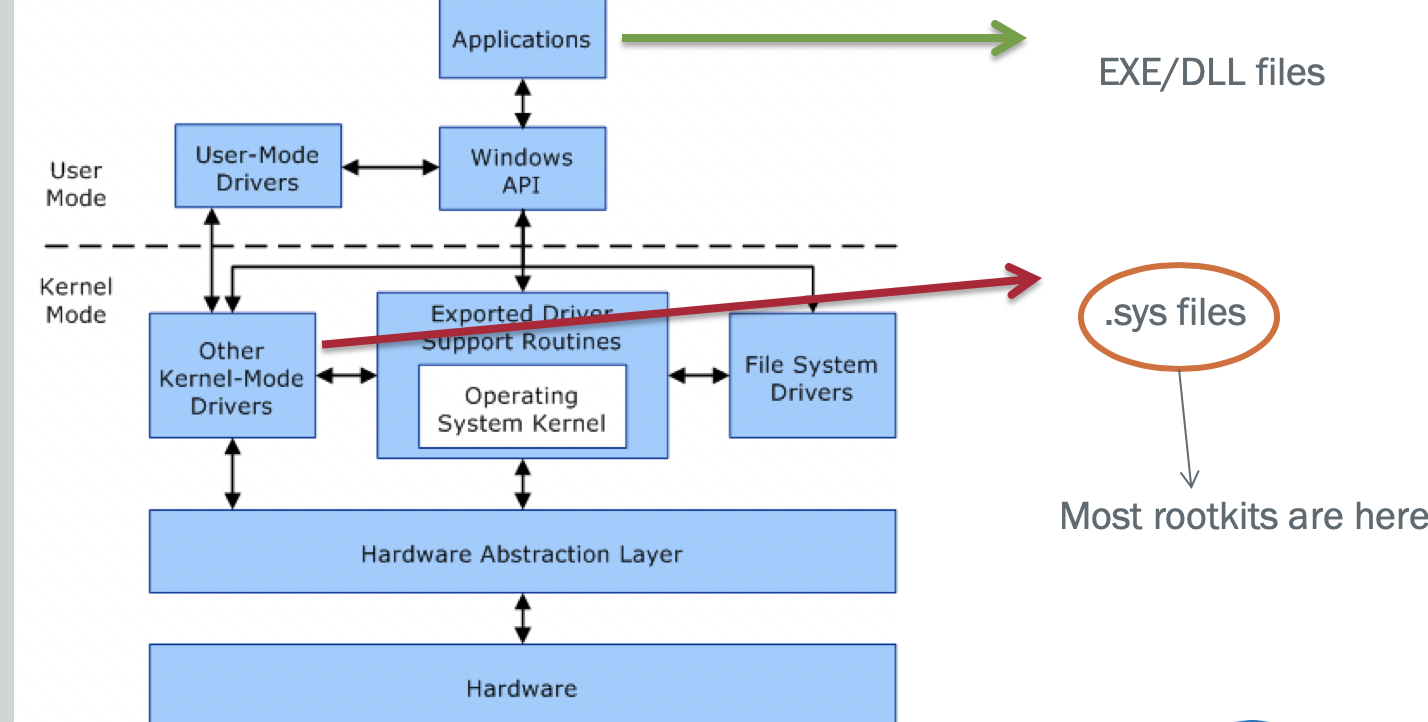
\includegraphics{1.png}
\item Kernal Memory is a flat memory model with no security separation
\item Any kernel driver can access any part of memory
\item Composed of windows kernel (ntoskmi.exe) as well as driver code
\item Many important structures that are prime targets for stealth – SSDT, IRP, IDT
\item Windbg commands: .process command, lm, !devobi, !drvobj, !devstack, tirp, etc. Virtual to physical memory
\item Lab 1 – Agony – Quick & high-level analysis. Cuckoo and memory malipulation
\item Thread Basics: HLL-Assembly-Machine Code (HEX)-RAM-BUS-instruction pipeline
\item CPU Hyperthreading

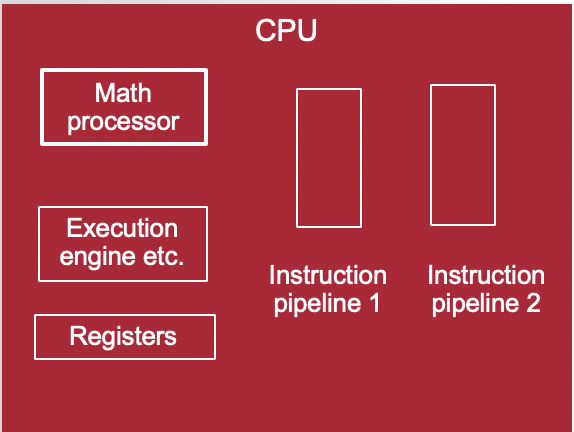
\includegraphics{2.png}
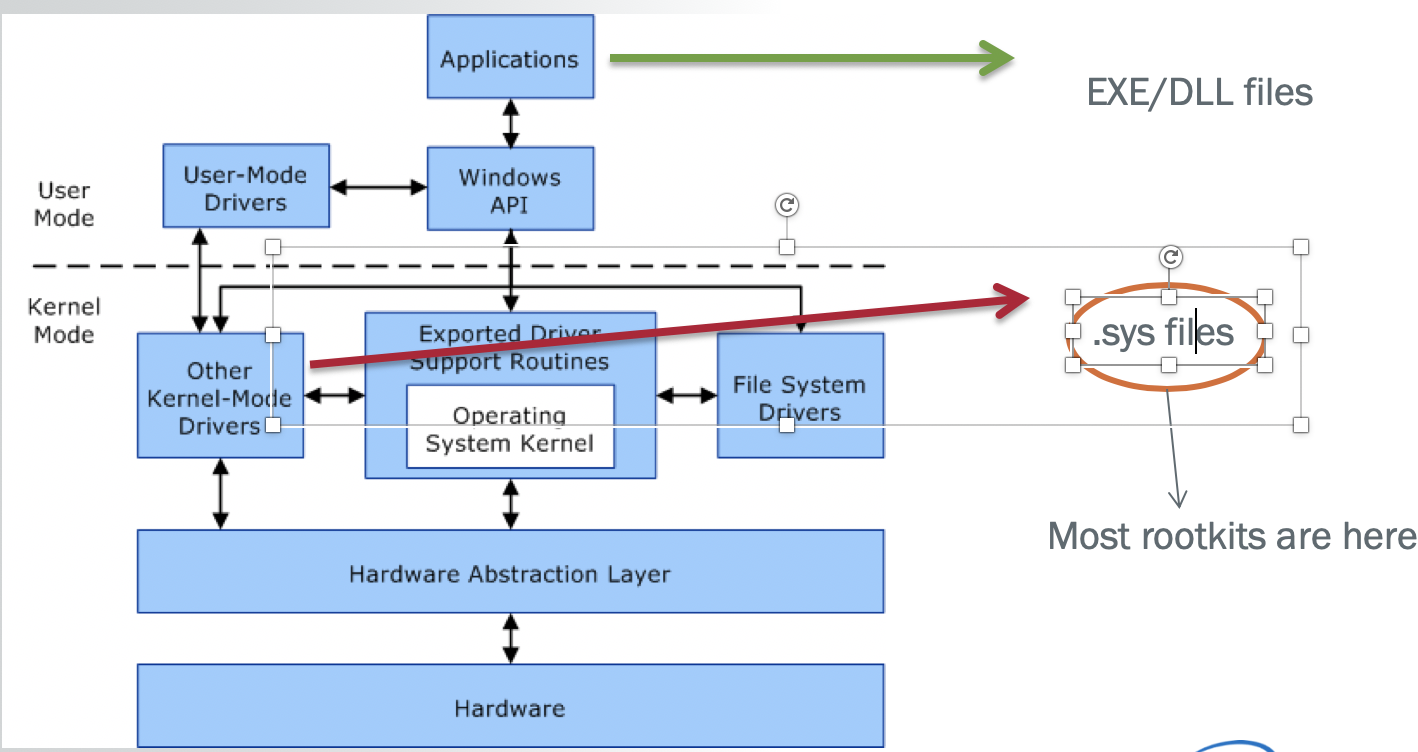
\includegraphics{3.png}

\item Threads is the smallest ‘unit’ of execution that can execute code
\item Thread context, stack, environment block (TEB), scheduling, Thread-process relationship
\item Thread object defines a thread: Kernal objects are data structure defined by OS to describe various OS constructs, thread being one such construct
\item Thead context stores all the related register values of the thread. During execution register values are stored in CPU, else they are in Memory.
\item Each Thread has its own stack: user mode stack, kernel stack
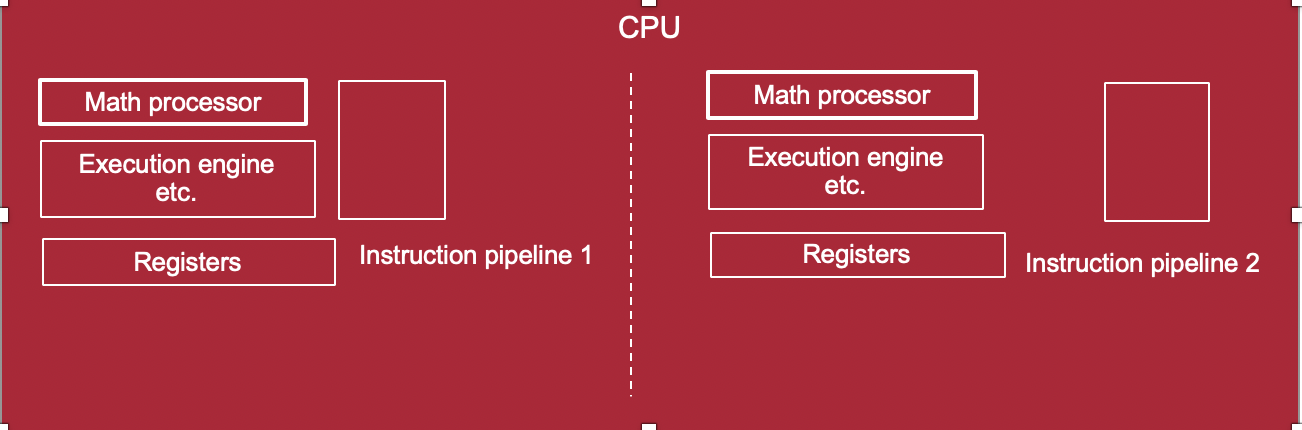
\includegraphics{4.png}
\item Process memory: Tool (Process hacker)
\item Processes are implemented as objects
\item An executable process may contain one or more threads
\item Process includes an object table that has handles to other objects known to this process.
\item A process needs at least one thread to execute
\item Lab 2 – Peering into Process Memory
\item Hooking Basics
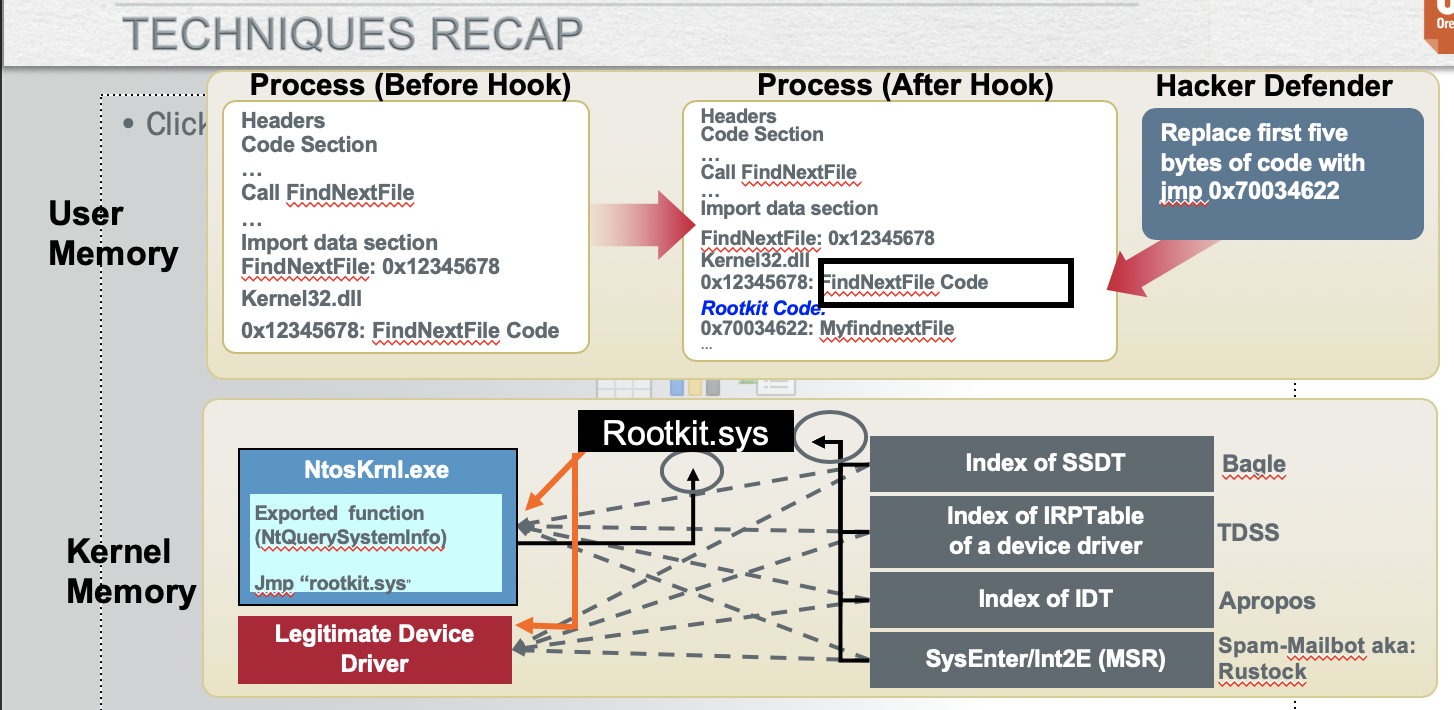
\includegraphics{5.png}
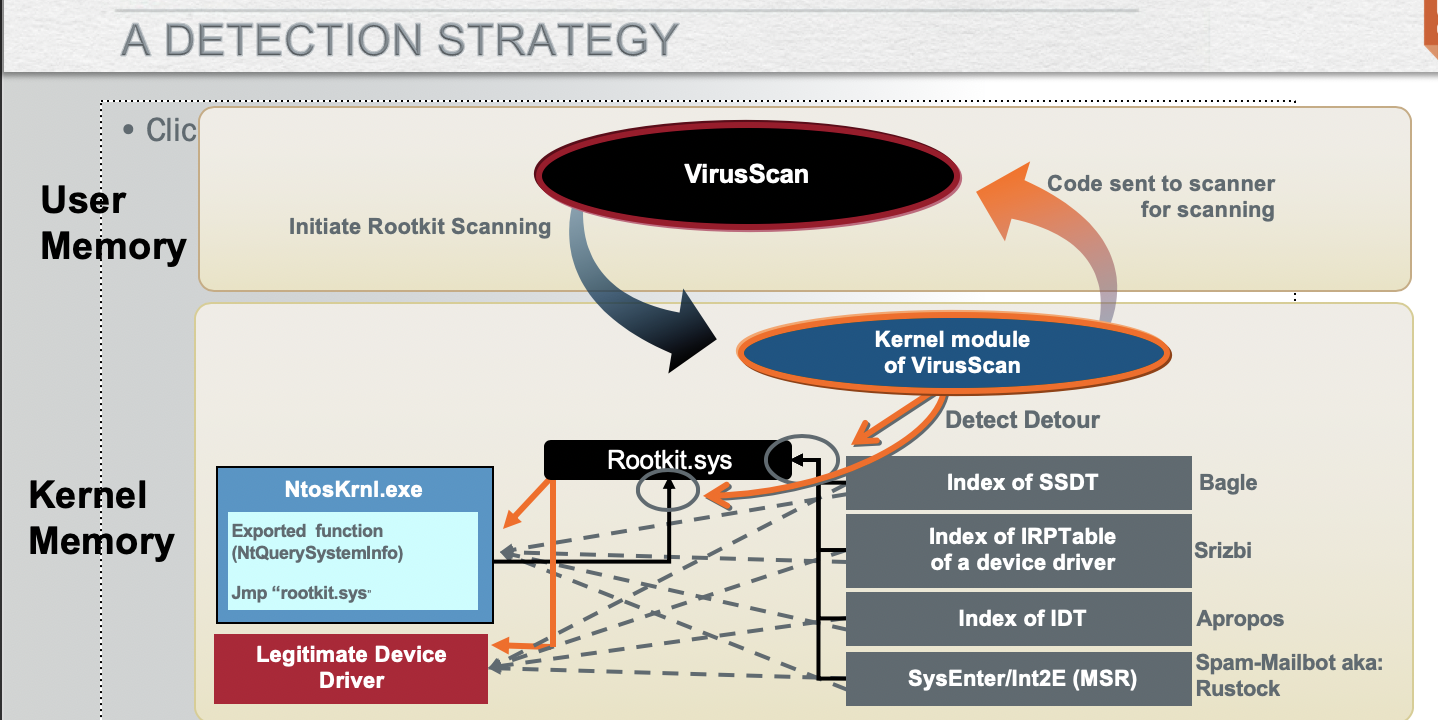
\includegraphics{6.png}
\item Lab 3 – Kernal debugging 101
\item Cekno Analysis & Detection
\item Kernal debugging is more powerful than merely using liveKD
\item Finding memory patterns and following the pointers in memory
\item Kernal debugging is like any other program debugging you do in your HLL code
\item Two machines – one a debugger and another debugee – talking to each other via virtual serial ports
\end{itemize}

\newline
Day 2
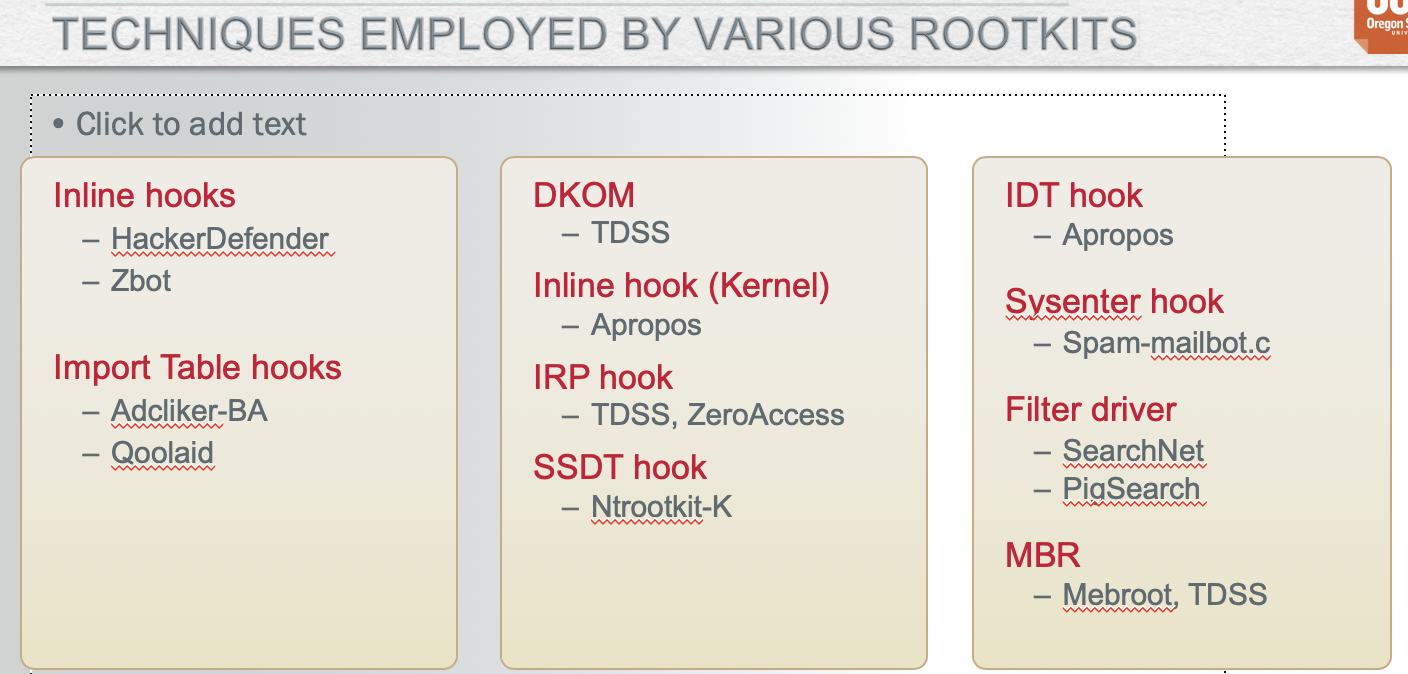
\includegraphics{7.png}
\begin{itemize}
\item System boot process
\item Pre-boot – power on self test to diagnose memory, hardware components, it loads the BIOS that locates the boot devices an dthne loads and runs MBR
\item Boot – initial boot loader, OS selection. MBR finds the active partition and load the boot sector in memory to execute it. Boot sector loads the NTLDR from disk 
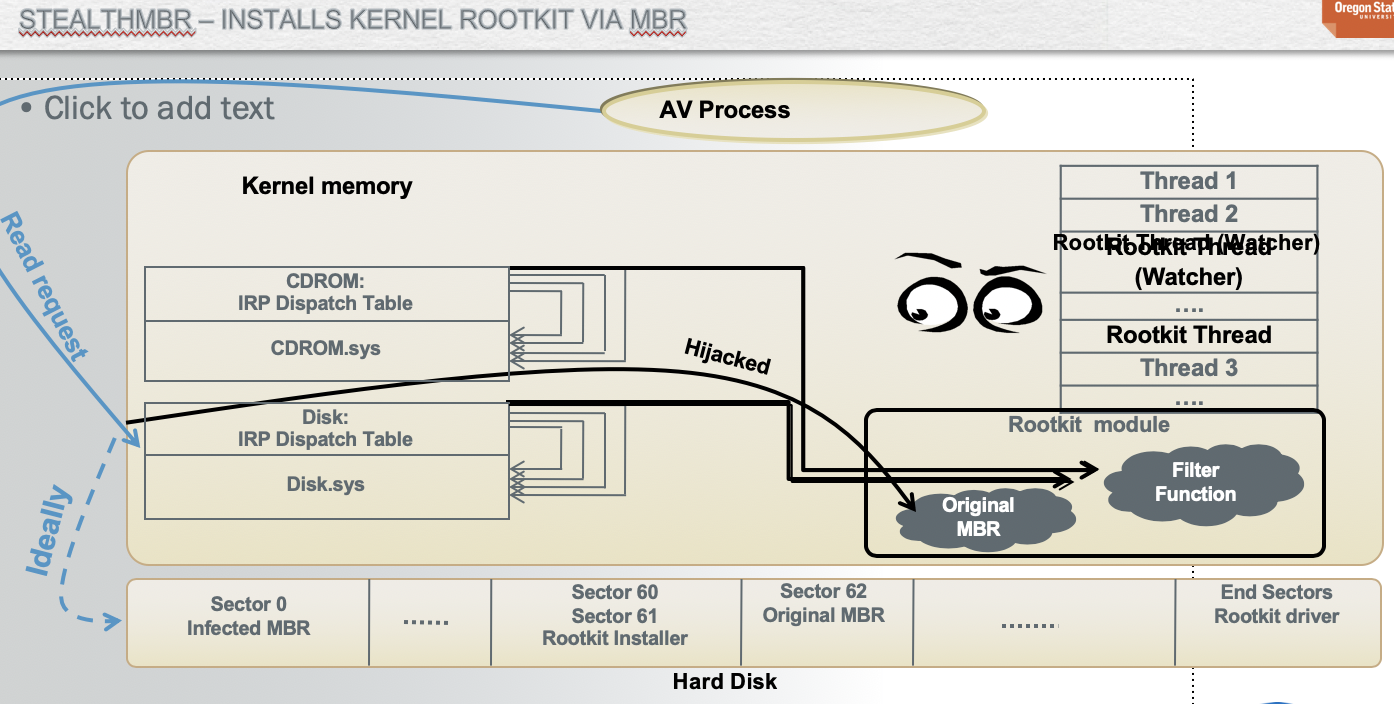
\includegraphics{8.png}
\item Lab 4 – Kernal Structure Analysis
\item Trends in Stealth Analysis – File forging, memory forging, self protection, attack AV, disassociating memory from file-on-disk, removing dependency on files, untrusting the trusted
\item Disassociating memory from file-on-disk. Rootkit’s memory can give-away its associated file on disk. Memory scanner needs to know the file. But can be difficult to track kernel memory.
\item File Content Foraging – overwrite existing files and forge the ‘view; such as the AV gets the clean view instead of the malicious. Better than hiding files
\item Removing dependency on files – scanners based on direct file-system (FS) parses worked well. So having no file in the FS helps rootkits, so move malicious code to boot process or BIOs and move encrypted malicious code to raw sectors or as a file. Advantages in 64-bit Windows
\item From limited self preservation – defend components and/or attack security components. Watcher threads (monitor and protect memory hooks and disk changes, rewrite registry, files, gain exclusive locks from SYSTEM), and attachs from kernel (callback registration to attack during process, module load)
\item Holistic Self Defenses – Behavior ID of AV, untrusting the AV and whitelisting of legitimate applications
\item Lab 5 – Analyze banker rootkit
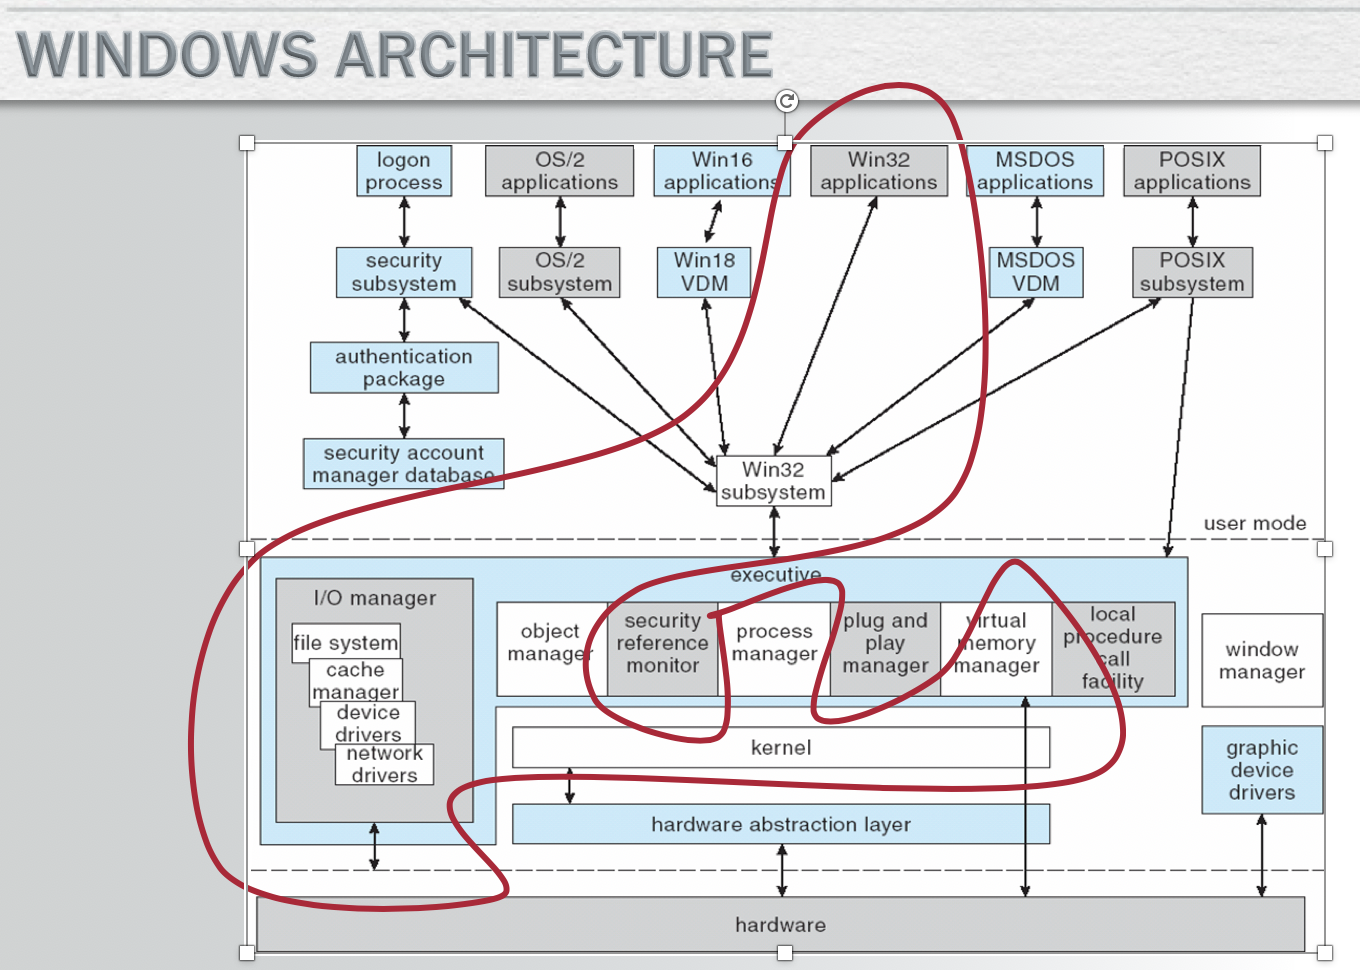
\includegraphics{9.png}
\end{itemize}
% --------------------------------------------------------------
%     You don't have to mess with anything below this line.
% --------------------------------------------------------------
 
\end{document}
